% !TeX program = lualatex

\documentclass[
	ngerman,
	color = black,
	]{tudaexercise}

\usepackage[english, main=ngerman]{babel}
\usepackage[autostyle]{csquotes}
\usepackage{inputenc}

\usepackage{amsmath}
\usepackage{amsfonts}
\usepackage{amssymb}

\usepackage{siunitx}

\usepackage{float}

\usepackage{graphicx}
%\usepackage[left=1cm,right=1cm,top=0.5cm,bottom=0.5cm]{geometry}
\usepackage{tikz}
\usepackage{tikz-3dplot}

\usepackage{multicol} % For pictures side by side

\usetikzlibrary{decorations.markings}
\usetikzlibrary{patterns}

%%%%%%%%%%%%%%%%%%%%%%%%%%%%%%%%%%%%%%%%%%%%%%%%%%%
% hacked version of usetikzlibrary to work around writeLaTeX file naming
% restrictions:
\makeatletter
\def\underscoreusetikzlibrary{\pgfutil@ifnextchar[{\underscoreuse@tikzlibrary}{\underscoreuse@@tikzlibrary}}%}
\def\underscoreuse@tikzlibrary[#1]{\underscoreuse@@tikzlibrary{#1}}
\def\underscoreuse@@tikzlibrary#1{%
	\edef\pgf@list{#1}%
	\pgfutil@for\pgf@temp:=\pgf@list\do{%
		\expandafter\pgfkeys@spdef\expandafter\pgf@temp\expandafter{\pgf@temp}%
		\ifx\pgf@temp\pgfutil@empty
		\else
		\expandafter\ifx\csname tikz@library@\pgf@temp @loaded\endcsname\relax%
		\expandafter\global\expandafter\let\csname tikz@library@\pgf@temp @loaded\endcsname=\pgfutil@empty%
		\expandafter\edef\csname tikz@library@#1@atcode\endcsname{\the\catcode`\@}
		\expandafter\edef\csname tikz@library@#1@barcode\endcsname{\the\catcode`\|}
		\catcode`\@=11
		\catcode`\|=12
		\input tikzlibrary\pgf@temp_code.tex
		\catcode`\@=\csname tikz@library@#1@atcode\endcsname
		\catcode`\|=\csname tikz@library@#1@barcode\endcsname
		\fi%
		\fi
	}%
}
\makeatother
%%%%%%%%%%%%%%%%%%%%%%%%%%%%%%%%%%%%%%%%%%%%%%%%%%%

\underscoreusetikzlibrary{mec}


\ConfigureHeadline{
	headline={Name:  Matrikelnummer: }
}

\begin{document}

\title[Übung TUDaExercise]{Klausur Grundlagen des CAE/CAD}
%\subtitle{Untertitel}
\author{Prof. Dr.-Ing. R. Anderl}
\term{Wintersemester 2021}
\date{17.04.2021}

\maketitle

% Aufgabe 1
\begin{task}[credit=13 P]{Geometriemodelle}
	\begin{subtask}[credit=4 P]
		Das abgebildete Bauteil wurde mit verschiedenen Features (Konstruktionselementen) modelliert.
		Benennen Sie die einzelnen Features und tragen Sie diese unter Berücksichtigung der Reihenfolge (vom Groben ins Feine) in die untenstehende Liste eindeutig ein, sodass eine Zuordnung der Features zur Geometrie möglich ist.
		
		\textit{Hinweis: Keine Features auf der Rückseite.}
		% 7 Linien
		\begin{multicols}{2}
			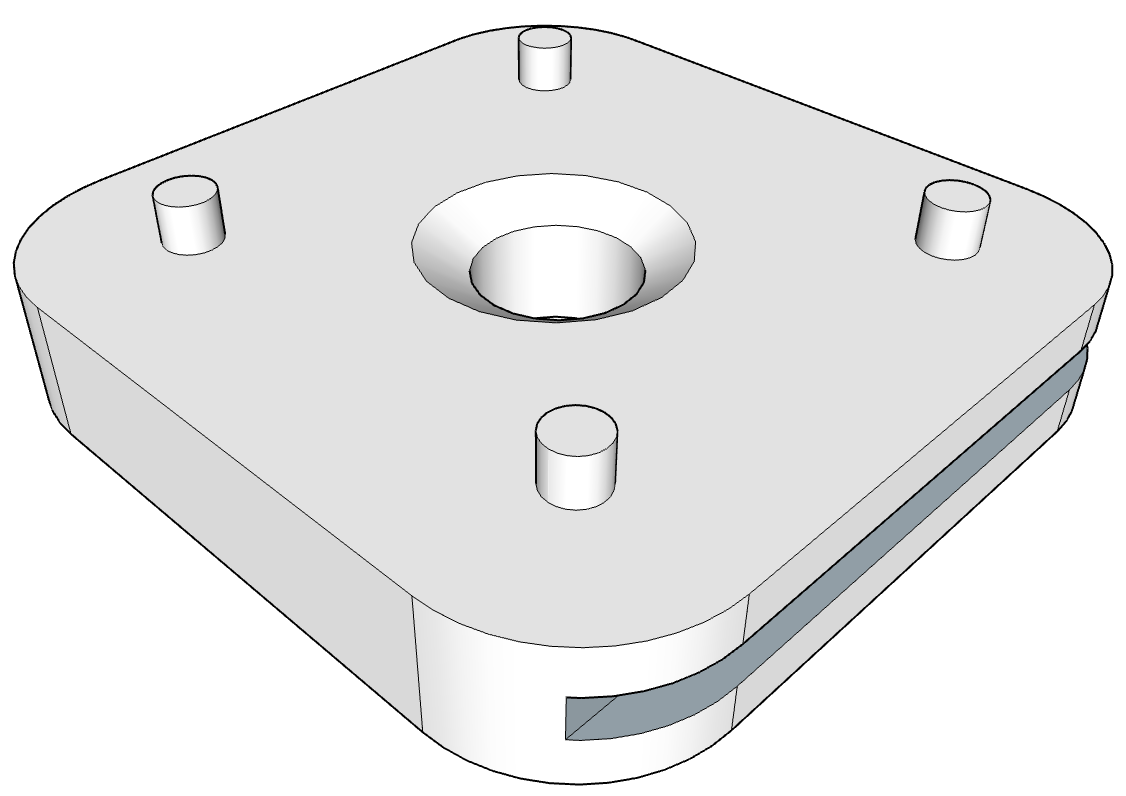
\includegraphics[width=.5\textwidth]{Grdl_Klausur_A1a.png}
			\columnbreak
			\begin{itemize}
				\item \rule{8cm}{0.15mm}
				\item \rule{8cm}{0.15mm}
				\item \rule{8cm}{0.15mm}
				\item \rule{8cm}{0.15mm}
				\item \rule{8cm}{0.15mm}
				\item \rule{8cm}{0.15mm}
				\item \rule{8cm}{0.15mm}
			\end{itemize}
		\end{multicols}
		
	\end{subtask}
	
	\pagebreak
	
	\begin{subtask}[credit=9 P]
		Erstellen sie anhand der unten gegebenen Volumenprimitiven (\textbf{Q}uader und \textbf{Z}ylinder) den CSG-Baum für das abgebildete Bauteil.
		Verwenden Sie bekannte mengentheoretische Operatoren.
		
		\begin{multicols}{2}
			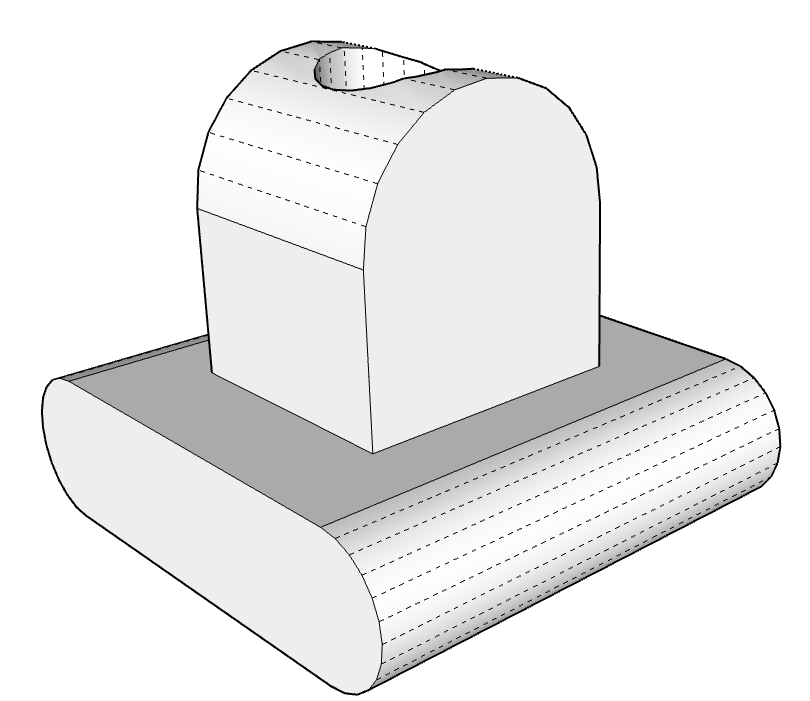
\includegraphics[width=.5\textwidth]{Grdl_Klausur_A1b.png}
			\columnbreak
			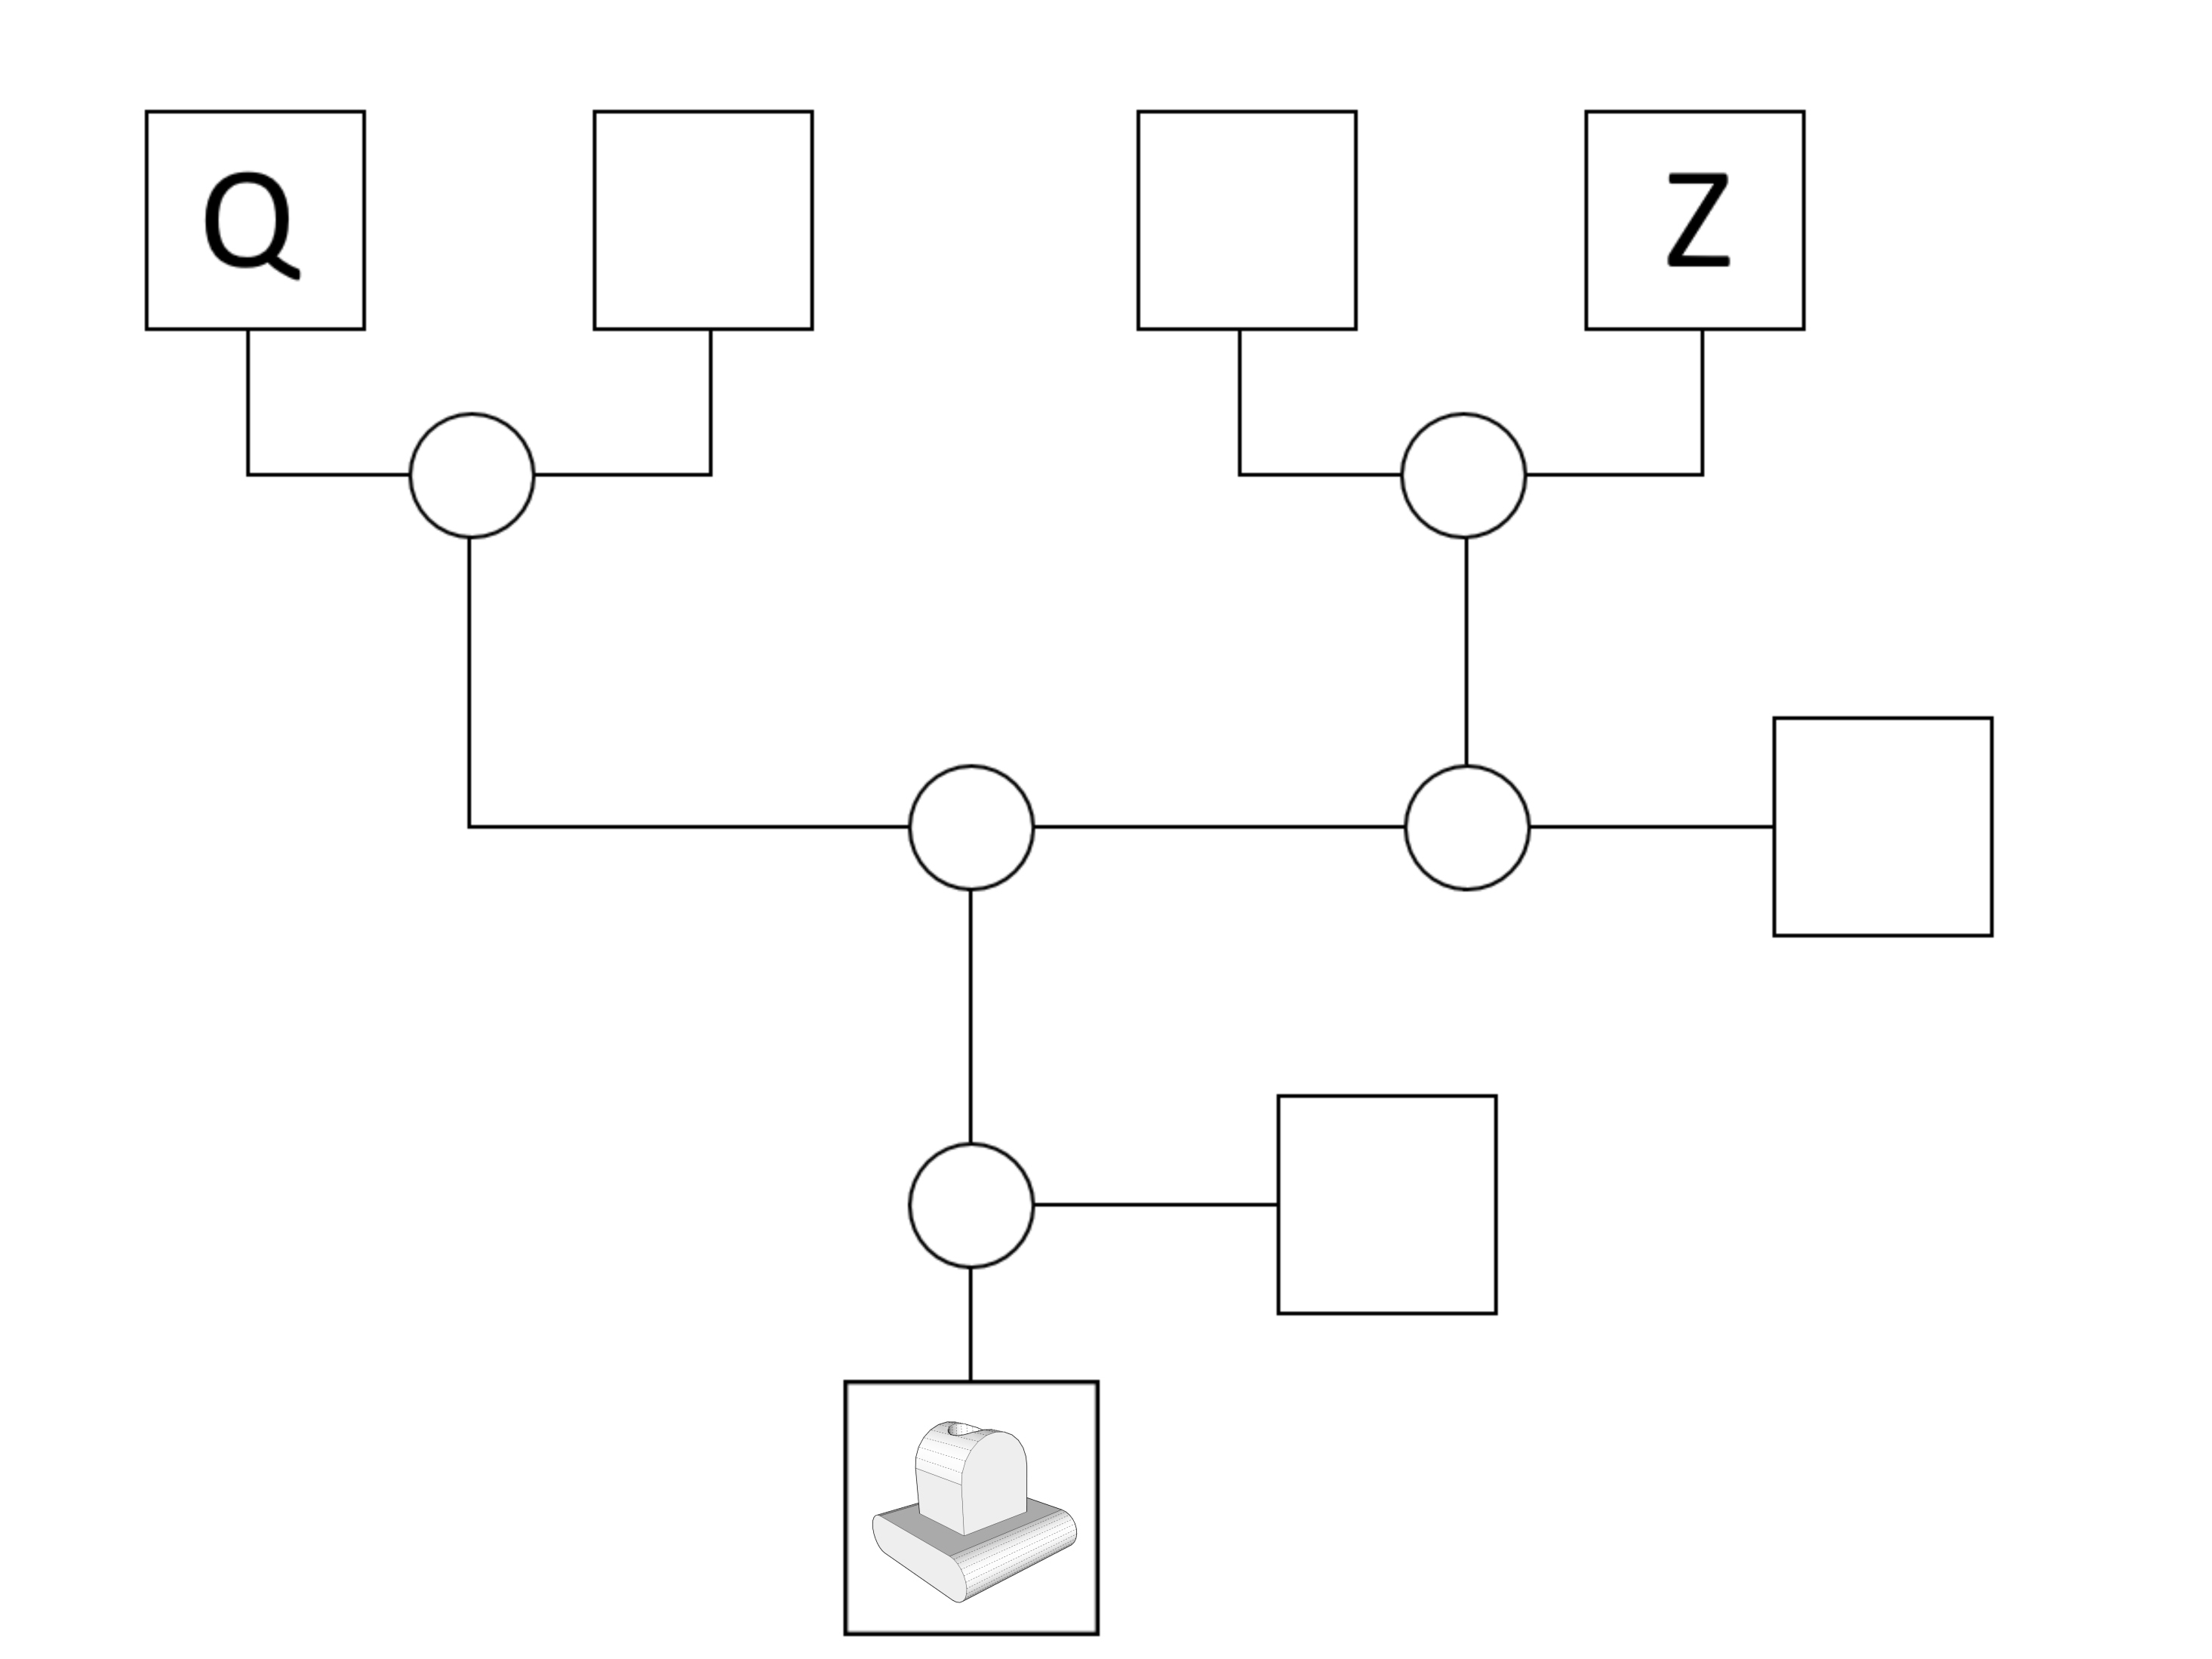
\includegraphics[width=.5\textwidth]{Graph-b-smaller.png}
		\end{multicols}
	\end{subtask}

	
\end{task}

% Aufgabe 2
\begin{task}[credit=21 P]{Geometrische Modellierung und Volumenmodelle}
	\begin{subtask}[credit=6 P]
		Nennen Sie die Merkmale geometrischer Modellierung.
		Verwenden Sie das gelernte Ordnungsschema.
	\end{subtask}
	
	\begin{subtask}[credit=2{,}5 P]
		Ein wichtiges Geometrieelement sind die Freiformkurven.
		Welche Freiformkurven wurden im Rahmen der Vorlesung behandelt und in welche 2 Kategorien lassen sich die Kurven unterscheiden.
	\end{subtask}
	
	\begin{subtask}[credit=1{,}5 P]
		Welche Möglichkeiten zur Beeinflussung der Kurve gibt es für Hermitkurven?
		Skizzieren sie ein Beispiel.
	\end{subtask}
	
	\begin{subtask}[credit=6 P]
		Volumenmodelle sind in der Lage Volumina vollständig zu beschreiben und Körper zu definieren.
		Nennen Sie die verschiedenen Volumenmodelle basierend auf den unterschiedlichen Datenstrukturen.
		Beschreiben Sie jedes Volumenmodel in einem Satz.
	\end{subtask}
	
	\begin{subtask}[credit=5 P]
		Im Rahmen der Volumenmodelle ist der Unterschied zwischen Geometrie und Topologie wichtig.
		Wie sind diese Begriffe definiert?
		Stellen Sie die jeweiligen Elemente in einem Schaubild gegenüber.
	\end{subtask}
	
\end{task}

% Aufgabe 3
\begin{task}[credit=9 P]{Geometrische Modellierung}
	\begin{subtask}[credit=2 P]
		geometrische Transformation im 3d Raum; Wieso 4*4 und ...
	\end{subtask}
	
	\begin{subtask}[credit=2 P]
		Stellen Sie die Matrizen für die Translation und Rotation um die y-Achse auf.
	\end{subtask}
		
	\begin{subtask}[credit=3 P]
		Translieren Sie den Punkt (1,7,4) um $d_x=1$, $d_y=3$ und $d_z=4$.
	\end{subtask}
	
	\begin{subtask}[credit=2 P]
		Drehen Sie das Ergebnis von voriger Aufgabe 30° um die z-Achse.
	\end{subtask}
\end{task}

% Aufgabe 4
\begin{task}[credit=15{,}5 P]{Datenmanagementsysteme}
	% Reihenfolge?
	\begin{subtask}[credit=5 P]
		 Produktrepräsentationen von Einzeltteilmodellierung, CFD, FEM, RPT CAD/CAM
	\end{subtask}
	
	\begin{subtask}[credit=2 P]
		
	\end{subtask}
	
	\begin{subtask}[credit=2{,}5 P]
		Was sind Inputdeck und Outputdeck und welche Daten enthalten diese?
	\end{subtask}
	
	% Aus Skript so ungefähr zur Einleitung:
	Unterschiedliche Gründe für den Einsatz von Produktdatenmanagementsystemen sowie deren konkrete Einsatzziele ergeben sich aus den Zielgrößen der Produktentwicklung:
	\begin{itemize}
		\item Erhöhung der Produktqualität
		...
	\end{itemize} %?
	
	\begin{subtask}[credit=4 P]
		Welche wichtigen Funktionsbestandteile haben Produktdatenmanagementsysteme?
		Nennen Sie die unterschiedlichen Ziele beim Einsatz von PDM-Systemen, sowie in welchen Teilbereichen diese Methoden zu einer Verbesserung führen.
	\end{subtask}
	
	\begin{subtask}[credit=2 P]
		Nennen Sie zwei Beispiele der Verwendung von Metadaten in SDM.
	\end{subtask}
\end{task}

% Aufgabe 5
\begin{task}[credit=18{,}5 P]{CAE-Prozessketten}
	% Reihenfolge?
	\begin{subtask}[credit=2 P]
		Ordnen Sie die folgenden Lastfälle den "Prozessen" zu:
		MKS, FEM x2, CFD, Kräfte/Momente, Druck, Bewegungsbahn, Temperatur
		Strömungsimulation, Bewegungsabläufe, Temperaturverteilung/ Wärmeübertragung, Strukturmechanik %ähnlicher Wortlaut
	\end{subtask}
	
	\begin{subtask}[credit=4 P]
		Unterscheidungskriterium für MKS Simulationen und in welche 2 Arten die Mehrkörper analyse unterteilt werden
		+ 3 Anwendungsfälle %?
	\end{subtask}	
	
	\begin{subtask}[credit=4 P]
		FEM-Prozesskette als Stichpunkte
		% welche verfahren es zur netzerstellung von fe gibt
	\end{subtask}
	
	\begin{subtask}[credit=2{,}5 P]
		Welche Randbedingungen können in der CFD angegeben werden?
	\end{subtask}
	
	\begin{subtask}[credit=4 P]
		
	\end{subtask}
	
	\begin{subtask}[credit=2 P]
		Nennen sie die beiden Formulierungen in der CFD (Netzgenerierung)
	\end{subtask}
\end{task}

% Aufgabe 6
\begin{task}[credit=23 P]{FEM}
	\begin{subtask}[credit=5 P]
		Nennen Sie die Berechnungsschritte, die zur Berechnung der an Knoten wirkenden Kräfte mittels der FE-Methode durchgeführt werden müssen.
		Beachten Sie dabei auch die Reihenfolge.
	\end{subtask}
	
	
	\begin{figure}[H]
		\centering
		\begin{tikzpicture}[node distance=1mm]
			\coordinate (a) at (1,1);
			\coordinate (b) at (1,4);
			\coordinate (c) at (4,1);
			
			\node[draw, hinge, grounded] (A) at (a) {};
			\node[draw, support, grounded] (C) at (c) {};
			
			\draw[black] (A) node[left] {$1$} -- (b) node[left] {$2$} -- (C) node[right] {$3$} -- (A);
			\draw[black] (2.5,1) node[above] {$(1)$};
			\draw[black] (1,2.5) node[right] {$(2)$};
			\draw[black] (2.6,2.3) node[left] {$(3)$};
			
			\draw[<->] (1,2) node[left] {y} -- (1,1) -- (2,1) node[below] {x};
		\end{tikzpicture}
		\label{fig:quer}
	\end{figure}
	
	\begin{subtask}[credit=2 P]
		Geben Sie die Federkonstante $k_i=\frac{EA}{L_i}$ der drei Stäbe in Abhängigkeit der gegebenen Größen E, A und L an.
		Beachten Sie $L_1 = L, L_1 \ne L_2 = L_3$.
	\end{subtask}
	
	Zur Ermittlung der wirkenden Kräfte muss das Gleichungssystem $f = K * u$ gelöst werden.
	
	\begin{subtask}[credit=16 P]
		Ermitteln Sie die globale Steifigkeitsmatrix $\mathbf{K}$ für das gegebene Stabwerk.
		Dokumentieren Sie Zwischenergebnisse.
		Beachten Sie das gegebene Koordinatensystem.
		Nehmen Sie nur für diesen Aufgabenteil für die Federkonstante an: $k_1 = k_2 = k_3 = k$.
		\textit{Hinweis: Das Lösen der Meister Zahlenwerte run}
	\end{subtask}
\end{task}

\end{document}
